\chapter{Datový model}
	Tato kapitola se zabývá podrobnostmi o datovém modelu. Pojednává o volbě reprezentace kontraktů, které byly použity pro tento projekt a obecně o společných atributech kontraktů. Jsou zde uvedeny podrobnosti o datovém modelu určeném pro reprezentaci kontraktů, ale také pro výsledky jejich porovnání. Oba tyto modely jsou zde popsány slovně, ale i pomocí UML diagramu. Závěr tvoří informace o externí reprezentaci těchto dat.

	\section{Volba DbC konstrukcí}
		Po analýze dostupných materiálů jsem se rozhodl zvolit pro implementaci konstrukce Guava Preconditions a JSR305. Důvodem byla především jejich rozdílná reprezentace, kdy Guava Preconditions je realizováno pomocí volání metod uvnitř těl metod, tedy se jedná o knihovnu, která zprostředkovává API. Avšak Guava Preconditions umožňuje tvorbu pouze vstupních podmínek.\\
		
		 Na druhé straně JSR305 je tvořené anotacemi v záhlaví tříd, metod a také jako součást parametrů metod. Umožňuje tvoření všech tří typů kontraktů (vstupní, výstupní i neměnné podmínky). Kromě této diverzity se také jedná o jedny z častých konstrukcí používaných v projektech viz \cite{contractsInWild}. Principy obou těchto nástrojů byly již popsány výše (viz 3. kapitola Popis kontraktů softwarových rozhraní), z čehož se bude vycházet.
				
				
	\section{Společné znaky reprezentací kontraktů}		
		Při rozboru jednotlivých nástrojů pro reprezentaci design by contract zjistíme, že sdílejí mnoho podobných aspektů, které jsou klíčové pro vytvoření obecného modelu, který je schopen zachytit libovolnou konstrukci kontraktu.\\ 
		
		Do modelu je třeba nejprve zanést, o jaký nástroj pro práci s kontrakty se jedná (Guava, JSR305, atd.). Každý kontrakt je také vždy definován jedním ze tří typů podmínek (vstupní, výstupní a neměnná), to je také velmi důležitá informace, kterou je třeba do modelu zaznamenat. Kontrakty jsou také typicky definovány funkcí, která určuje, co kontrakt ověřuje. Může se jednat o kontrolu argumentu, zda objekt není \texttt{null} atp. V případě, že kontrakt tuto informaci neobsahuje, může tato položka zůstat prázdná.\\
		
		Další důležitou informací je hodnota daného kontraktu, která představuje výraz, který je vyhodnocován. Některé kontrakty tuto hodnotu nevyžadují (např. \texttt{@Nonnull} u JSR305), ale ve většině případů jde o podmínku (např. \texttt{x > 0}). Některé druhy reprezentací kontraktů však umožňují i další argumenty. Typicky se jedná o informace o typu výjimky, která je vyhozena, či o její zprávě. Může se však také jednat o další upřesňující data. Obvykle tyto informace nemají z hlediska důležitosti vysokou prioritu, přesto by ale mělo být možné je do modelu zahrnout.
		
	
	\section{Model pro extrakci kontraktů}
			Aby bylo možné kontrakty extrahovat ze zdrojových souborů, je také třeba mít k dispozici datový model, do kterého bude možné tato data uložit. Tento model jsem vytvořil na základě analýzy konstrukcí kontraktů s ohledem na následný export do formátu dat, který bude možné dále zpracovávat. Aby byl zachován kontext kontraktů, usoudil jsem, že bude třeba ukládat také informace o třídách a metodách v daném souboru.\\
			
			Rozhodl jsem se tedy vytvořit strukturu podobnou stromu, jejíž kořenem je samotný zdrojový soubor (třída \texttt{JavaFile}). Tento soubor obsahuje různé podrobnosti o tomto souboru jako je jeho jméno a cesta, typ a statistiky o jeho obsahu. Také obsahuje seznam všech tříd (třída \texttt{JavaClass}) obsažených v tomto souboru.\\
			
			Každá jednotlivá třída pak obsahuje jméno, svou hlavičku, seznam metod (třída \texttt{JavaMethod}) a také seznam všech kontraktů týkajících se této třídy, tedy neměnných podmínek. Metoda pak nese informaci o své signatuře a také seznam všech kontraktů (třída \texttt{Contract}) dané metody. Samotný kontrakt pak obsahuje informaci o tom, o jaký typ kontraktu a podmínky se jedná, kompletní výraz a také jeho dílčí části (viz podrobnosti níže).\\
			
			V projektu je model reprezentován v rámci knihovny nástroje. Je zde balíček \texttt{model}, kde se nacházejí všechny zmíněné třídy.\\
			
			Na obrázku \ref{modelExtractorDiagram} je vidět grafické znázornění datového modelu formou UML diagramu. Nejsou zde záměrně zobrazeny objekty \texttt{ContractComparison} a \texttt{JavaFileCompareReport}. Těm je věnován prostor v diagramu pro porovnávání kontraktů, který je na obrázku \ref{modelComparatorDiagram}.\\ 
							
				\begin{figure}[!htb]
					\minipage{1\textwidth}	
						\centering
						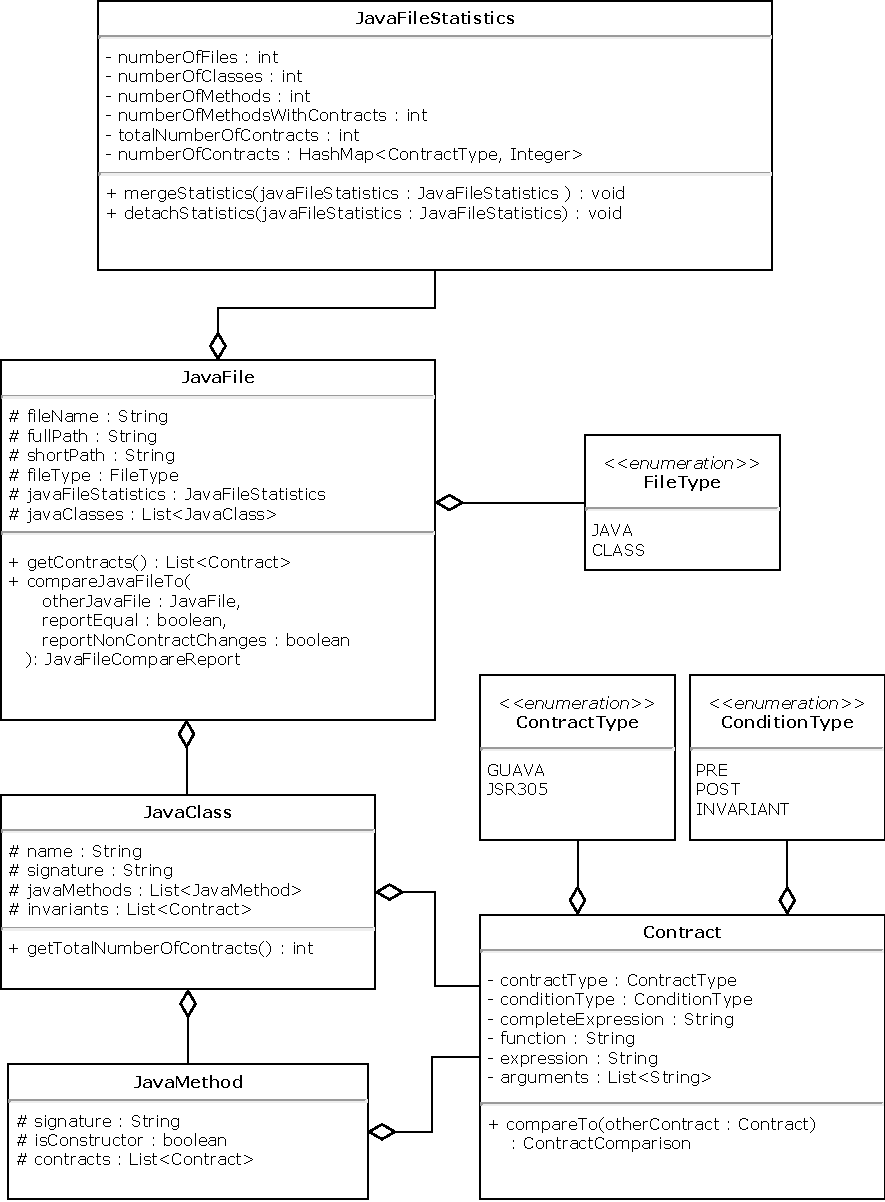
\includegraphics[width=1\textwidth]{img/modelExtractorDiagram.pdf}
						\caption[modelExtractorDiagram]{UML diagram datového modelu pro extrakci kontraktů}
						\label{modelExtractorDiagram}
					\endminipage\hfill
				\end{figure}				
			
			\subsection{Podrobností modelu}
				Následuje rozbor některých prvků modelu, které nemusejí být na první pohled samovysvětlující či je vhodné je vyzdvihnout kvůli své důležitosti.
				
				\subsubsection{Atribut \texttt{shortPath}}				
					Atribut \texttt{shortPath} ve třídě \texttt{JavaFile} slouží k zobrazení zkrácené cesty souboru, což zlepšuje přehlednost uživatelské aplikace. Pokud jsou přidány soubory ze stejné složky, které jsou hluboko v hierarchii souborového systému, název souboru by mohl být příliš dlouhý, aniž by poskytoval užitečnou informaci.\\
					
					Např. místo toho, aby byl soubor reprezentován dlouhou absolutní cestou \texttt{C:/test/guava-10.0/com/google/common/base/Objects.java}, zobrazí se pouze \texttt{base/Objects.java}. Jiný soubor pak může být reprezentován např. pomocí \texttt{util/concurrent/Atomics.java}. Zkrácená cesta se průběžně mění na základě přítomných souborů, aby bylo vždy možné je jednoznačně rozeznat. V případě potřeby, či aktualizace této cesty, je k dispozici absolutní cesta v atributu \texttt{fullPath}.
				
				\subsubsection{Třída \texttt{JavaFileStatistics}} 
					Atribut \texttt{totalNumberOfContracts} obsahuje informaci o celkovém počtu kontraktů nehledě na typ reprezentace. Naopak hash mapa \texttt{numberOfContracts} poskytuje celkový počet kontraktů pro daný typ reprezentace.\\
				
				Metody \texttt{mergeStatistics()} a \texttt{detachStatistics()} slouží ke sloučení respektive odloučení dané statistiky od aktivní statistiky. Tyto metody jsou využity při kalkulaci globálních statistik, kde je nutné provést aktualizaci vždy po přidání resp. při odebrání souborů.
					
				
				\subsubsection{Třída \texttt{Contract}}	
					Klíčovou částí celého modelu je jednoznačně třída \texttt{Contract}. Instance této třídy představují jednotlivé kontrakty souboru. Kontraktem je zde myšlena jedna vstupní, výstupní či neměnná podmínka doprovázena dalšími atributy. Následuje krátký popis a vysvětlení jednotlivých atributů této třídy.
					
					\paragraph{\texttt{ContractType contractType}} 
						Jedná se o výčtový typ, který určuje o jaký druh kontraktu se jedná. Při současném stavu knihovny to mohou být hodnoty Guava či JSR305.
			
					\paragraph{\texttt{ConditionType conditionType}} 
						Opět výčtový typ který určuje typ kontraktu dle jeho podmínky. Rozlišují se tři druhy: \texttt{PRE} pro vstupní podmínku, \texttt{POST} pro výstupní podmínku a \texttt{INVARIANT} pro neměnnou podmínku.
			
					\paragraph{\texttt{String completeExpression}} 
						Reprezentuje kompletní výraz celého kontraktu. I přesto, že celý výraz je možné vytvořit z jeho dílčích částí, je zde uveden pro rychlý přehled. Může také posloužit jako kontrola parsování či pro rychlé porovnání.
			
					\paragraph{\texttt{String function}} 
						Tento řetězec určuje funkci o jakou se jedná v rámci daného kontraktu. V případě Guava se jedná o název metody, v případě JSR305 o název anotace. Obecně se jedná o hlavní označení určující daný kontrakt.
			
					\paragraph{\texttt{String expression}} 
						Obsahuje první parametr dané funkce. Důvodem, proč oddělit první parametr od ostatních, bylo, že kontrakty mají často pouze jeden parametr a pokud jich mají více, ostatní často nejsou tolik relevantní. Pro zvýšení přehlednosti byl tedy tento parametr uveden samostatně.
			
					\paragraph{\texttt{List<String> arguments}} 
						Seznam ostatních argumentů daného kontraktu. Ostatní atributy až na výjimky slouží pouze k uvedení chybové zprávy, která se má zobrazit při porušení kontraktu. Mimo samotné zprávy zde také často bývají proměnné použité v šabloně zprávy.
					
				\subsubsection{Další třídy} 
					Během zpracování byly také používány následující třídy: \texttt{ExtendedJavaFile}, \texttt{ExtendedJavaClass} a \texttt{ExtendedJavaMethod}. Ty obsahují dodatečné informace vůči svým protějškům ve výše zmíněném modelu. Navíc obsahují informace o anotacích, vstupních parametrech a jednotlivých částech těl metod. Po zpracování jsou pak tyto objekty redukovány na ty výše zmíněné, které jsou připraveny pro externí reprezentaci.
		

	\section{Model pro porovnávání kontraktů}
		Vzhledem k tomu, že cílem nástroje nebyla pouze extrakce kontraktů, ale také jejich případné porovnání, bylo třeba vytvořit datový model, který umožní zachytit i tyto informace. Model jsem navrhoval s vědomím, že porovnání bude mít největší hodnotu ve chvíli, kdy bude možné porovnat kontrakty dvou projektů, tedy dvou složek. Samozřejmě nemá velký smysl porovnávat kontrakty dvou naprosto rozdílných projektů. Myšlenkou je porovnání dvou různých verzí téhož projektu. Pak je možné pozorovat, zda kontrakty přibývají či ubývají s rostoucím množstvím kódu a obecně různé trendy, které mohou poskytnout zajímavé informace o této problematice.\\ 
		
		S porovnáním dvou složek však také přibývá problém párování jednotlivých souborů, tříd, metod a kontraktů se svými protějšky v druhé složce. Na základě těchto informací jsem se tedy rozhodl, že hlavním objektem pro porovnání bude zpráva o rozdílech těchto dvou složek (projektů). Tato zpráva bude obsahovat různé podrobnosti o tom, zda byly složky shodné, konkrétní případy, kde se lišily a také seznam souborů, ke kterým nebyl nalezen adekvátní pár v druhé složce. Tím vzniká tedy seznam přidaných respektive odebraných souborů podobně jako u porovnávání dvou verzí při práci s VCS\footnote{VSC, neboli Version Control System je druh nástroje, který umožňuje týmu spravovat kód v průběhu času.}. Stejně jako v případě extrakce, i zde je souhrn statistik, který poskytuje dodatečné informace o tomto srovnání.\\
				
		Porovnání jednotlivých souborů jsou pak zachycena v objektu, který má podobné atributy jako ten pro složku, tedy v čem se dané soubory lišili z hlediska tříd, metod a zejména kontraktů. I zde je k dispozici souhrn statistik. Model by měl být patrný z z obrázku \ref{modelComparatorDiagram}, kde je tento model znázorněn graficky formou UML diagramu. Následuje také popis některých částí modelu, které nemusejí být na první pohled jasné, či se jedná o důležité prvky.\\
		
		V projektu je pak tento model opět součástí knihovny a nachází se v balíčku pro porovnávání (\texttt{comparator.comparatormodel}).
		
				\subsection{Podrobnosti modelu}
				
					\subsubsection{Atributy \texttt{apiEqual} a \texttt{contractEqual}}
						Tyto atributy určují, zda dvě složky či soubory jsou shodné z hlediska API respektive kontraktů. Atribut \texttt{apiEqual} tedy značí, zda jsou dané objekty shodné z hlediska definice tříd a jejich metod. Pokud například jeden soubor obsahuje metodu, kterou ten druhý nemá, či ji obsahuje, ale má pozměněnou signaturu, hodnotou \texttt{apiEqual} by bylo \texttt{false}.\\
						
						Atribut \texttt{contractEqual} značí, zda jsou dané objekty shodné z hlediska kontraktů. Tedy jestli jich obsahují stejný počet a zda jsou jednotlivé kontrakty shodné.
		
					\subsubsection{Třída \texttt{ApiChange}}
						Pomocí instancí této třídy je možné vyjádřit změny v API. Atribut \texttt{apiType} určuje, zda se změna týká třídy či metody. \texttt{apiState} pak určuje, zda byl daný element přidán, odebrán či tzv. \texttt{FOUND\_PAIR}. V tom případě se nejedná o změnu, ale naopak byl nalezen protějšek daného objektu. Pomocí instancí této třídy je pak vyjádřeno, které metody a třídy chybějí či se naopak nově objevily.
						
					\subsubsection{Třída \texttt{ContractComparison}}
						Tento výčtový typ představuje výsledek po porovnání dvou kontraktů. Může obsahovat tyto hodnoty:
						
						\paragraph{\texttt{EQUAL}}
							Tento výsledek značí, že jsou oba kontrakty naprosto shodné.
						
						\paragraph{\texttt{MINOR\_CHANGE}}
							Tento stav značí, že kontrakty jsou shodné, ale liší se v ostatních argumentech. Typicky se jedná o změnu zprávy o chybě či různá upřesnění. Z tohoto důvodu se jedná o \emph{minor change} (menší změnu).
							
						\paragraph{\texttt{SPECIALIZED}}
							Tímto tvarem je možné vyjádřit, že daný kontrakt je shodný jako ten druhý, nicméně má přísnější podmínku, je tedy více specializovaný. Triviálním příkladem může být situace, kdy první kontrakt má podmínku \texttt{x >= 0} a ten druhý podmínku \texttt{x > 0}. Zde je vidět, že druhá podmínka je přísnější. V současném stavu nástroje není tato hodnota používána, byla však připravena pro budoucí rozšíření.
							
						\paragraph{\texttt{GENERALIZED}}
							Jedná se o stejnou hodnotu jako \texttt{SPECIALIZED} s tím rozdílem, že je kontrakt naopak více obecný a má tedy mírnější podmínku. Stejně ani tento stav není momentálně využit.
							
						\paragraph{\texttt{DIFFERENT\_EXPRESSION}}
							Tímto stavem je vyjádřeno, že jsou dané kontrakty typově shodné, liší se však v atributu \texttt{expression}. Obvykle tedy platí, že liší v podmínce, či objektu, kterého se daný kontrakt týká. V současném stavu tento stav zahrnuje také stavy \texttt{SPECIALIZED} i \texttt{GENERALIZED}. Do budoucna by však stav \texttt{DIFFERENT\_EXPRESSION} měl být přípustný pouze pokud ani z dvou zmíněných stavů není možné prokázat (např. podmínku \texttt{y == 1} nelze porovnávat s podmínkou \texttt{x > 0}).
							
						\paragraph{\texttt{DIFFERENT}}
							Tento výsledek říká, že se oba kontrakty liší v některém ze základních atributů, tedy typ kontraktu či podmínky. Při porovnávání dvou souborů či složek by nemělo být možné tohoto stavu docílit, protože není možné nalézt pár k danému kontraktu, jestliže se takto výrazně liší. Důvodem tohoto stavu je zajištění úplnosti v případě porovnávání dvou kontraktů bez známého kontextu. 						 
							
		
				\begin{figure}[!htb]
					\minipage{1\textwidth}	
						\centering
						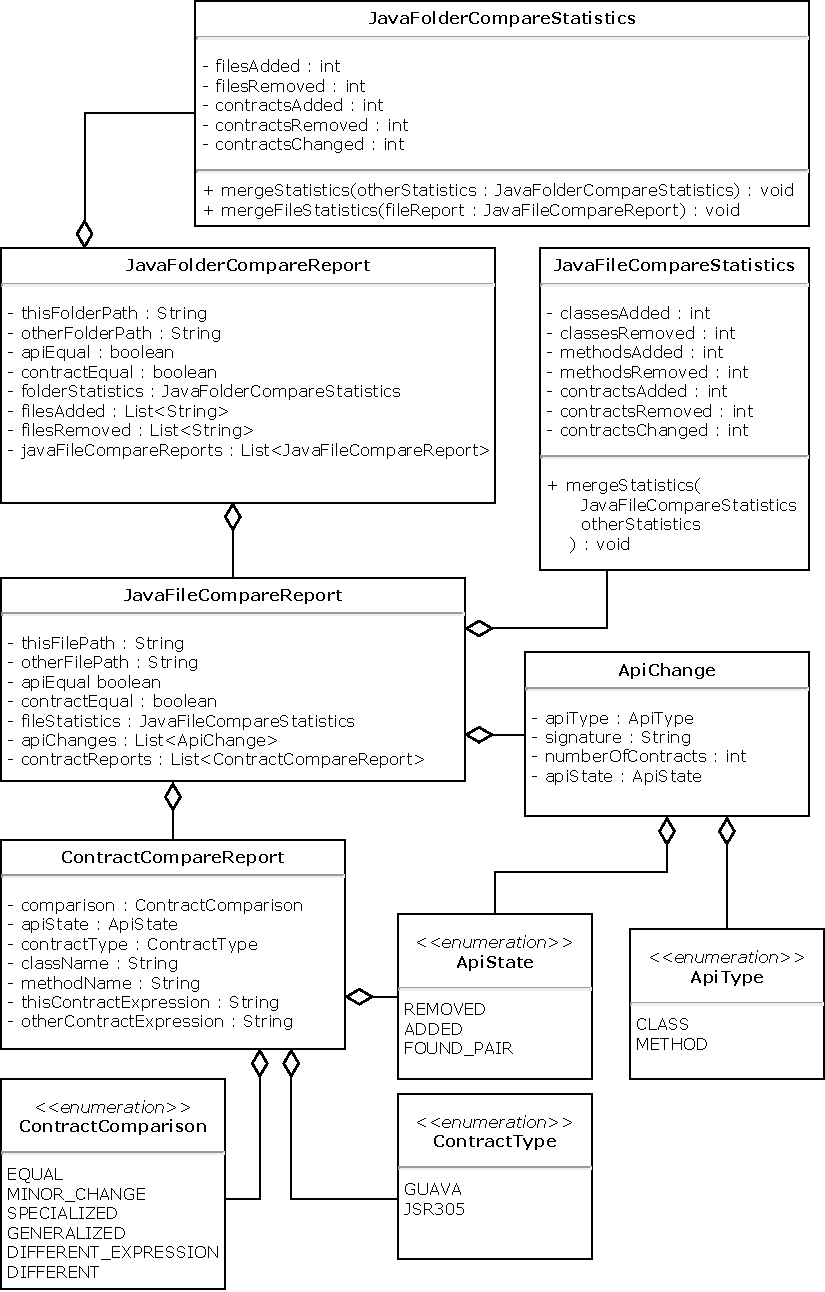
\includegraphics[width=1\textwidth]{img/modelComparatorDiagram.pdf}
						\caption[modelComparatorDiagram]{UML diagram datového modelu pro porovnání kontraktů}
						\label{modelComparatorDiagram}
					\endminipage\hfill
				\end{figure}

			
	\section{Externí reprezentace modelu}
		Pro externí reprezentaci modelu jsem zvolil použití formátu JSON. Tento formát je široce používaný zápis dat a umožňuje relativně snadné ukládaní objektů typu Java. JSON je tak vhodný pro zpracovaní strojem, ale je dobře čitelný i pro lidské oko (v případě, že byl zformátován). Díky těmto kvalitám je JSON vhodným formátem pro zobrazení, archivaci i další zpracování extrahovaných dat.\\
			
			Alternativou bylo použití formátu XML. Tento formát má v podstatě stejné přednosti jako JSON, s tím rozdílem, že obvykle není potřeba dalšího formátování proto, aby byl čitelný pro člověka, nicméně je oproti formátu JSON více opsaný. I přesto, že XML by byla také validní možnost pro reprezentaci dat, po dohodě s vedoucím práce jsme se rozhodli pro použití JSON. Důvodem byla zejména jeho stručnost, ale také lepší vlastnosti pro předávání mezi jinými nástroji.
			
		\subsection{Specifikace formátu}
			Formát JSON \cite{jsonSyntax} je velice jednoduchý a stručný. Objekty reprezentované v JSON jsou uzavřeny ve složených závorkách (\texttt{\{\}}), jelikož celý soubor vždy představuje jeden komplexní objekt, daný soubor vždy začíná i končí složenou závorkou. Názvy dílčích atributů jsou pak uzavřeny v uvozovkách a za dvojtečkou následuje jejich hodnota. Více atributů je pak odděleno čárkami.\\
			
			Daný atribut může mít přirozeně různé typy hodnot. Řetězce jsou standardně uvnitř uvozovek, čísla a výrazy \texttt{true/false} jsou pak bez uvozovek. Hodnotou však může být i další objekt či pole. Pole je uzavřeno v hranatých závorkách (\texttt{[]}) a položky jsou odděleny čárkami. Pokud je pole prázdné, jsou zde pouze obě závorky bez obsahu.\\
			
			Formát exportovaných souborů přímo vychází z výše zmíněných modelů. Daný soubor obsahuje tedy všechny objekty uvedené v modelu a je pouze převeden do formátu JSON. V následujícím příkladu je ukázka formátu souboru, který je vytvořen po extrakci kontraktů. Příklad je úmyslně zkrácen, v atributu \texttt{javaMethods} by standardně byly jednotlivé metody a v každé z daných metod pak případné kontrakty. Také by zde byly další atributy jako jsou statistiky, typ souboru atd.\\
							
			\noindent
			\- \- \- \texttt{\{}\\	
			\- \- \- \- \- \- \texttt{"fileName": "example.java", }\\
			\- \- \- \- \- \- \texttt{"fullPath": "C:/test/example.java", }\\ 
			\- \- \- \- \- \- \texttt{...}\\
			\- \- \- \- \- \- \texttt{"javaClasses": [}\\
			\- \- \- \- \- \- \- \- \- \texttt{\{}\\
			\- \- \- \- \- \- \- \- \- \- \- \- \texttt{"name": "Example"}\\
			\- \- \- \- \- \- \- \- \- \- \- \- \texttt{"signature": "public class Example"}\\
			\- \- \- \- \- \- \- \- \- \- \- \- \texttt{"javaMethods": [}\\
			\- \- \- \- \- \- \- \- \- \- \- \- \- \- \- \texttt{...}\\ 
			\- \- \- \- \- \- \- \- \- \- \- \- \texttt{],}\\
			\- \- \- \- \- \- \- \- \- \- \- \- \texttt{"invariants": []}\\
      		\- \- \- \- \- \- \- \- \- \texttt{\}}\\
      		\- \- \- \- \- \- \texttt{]}\\
      		\- \- \- \texttt{\}}\\			